\chapter{Anwendung des Frameworks auf jadice flow}
\label{chap:anwendung}

In diesem Kapitel wird ein Architektur-Refactoring am Produkt \jf geplant und in theoretischer Ebene durchgeführt.
Dazu werden das \acrfull{mmf} beziehungsweise der \acrfull{arh} verwendet, welche den Prozess in drei Phasen unterteilen.
Eine genauere Beschreibung des Frameworks ist in \cref{sec:mmf} zu finden.
Sehr abstrahiert und vereinfacht bestehen die Phasen aus den folgenden Aktivitäten:
\begin{itemize}
	\item In \cref{sec:durchführung-phase1} wird die Durchführung der ersten Phase in Form eines Architekturreviews mit den wichtigsten Stakeholdern beschreiben.
	\item Im Rahmen der zweiten Phase werden in \cref{sec:durchführung-phase2} Filter konfiguriert und anschließend adäquaten Migrationsstrategien gesucht.
	\item In \cref{sec:durchführung-phase3} wird in der dritten Phase eine Suche nach geeigneten \bpp beschrieben.
\end{itemize}

\section{Phase 1 - Systemverständnis}
\label{sec:durchführung-phase1}

Das Ziel der ersten Phase ist, ein Verständnis des Systems aufzubauen.
Das ist zum einen auf Seite der Stakeholder wichtig.
Diese sollten spätestens nach dieser Phase wissen, welche \acrfullpl{qa} besonders wichtig für das System sind.
Zum anderen sollte der \gls{arh} nach dieser Phase durch Eingabe der \glspl{qa} ein Verständnis des Systems erlangen, das er in den nächsten Phasen zur Unterstützung der Entwickler bei Migration verwenden kann.

Um diese Eingaben für den \gls{arh} zu generieren, wurde am 6. November 2023 ein Architekturreview wie in \cref{sec:methodik-architekturreview} beschrieben durchgeführt und am 14. November 2023 fortgesetzt.
Teilgenommen haben vier Softwareentwickler beziehungsweise -Architekten, der \acrlong{po} nach Definition des SCRUM von \Citet{SCRUM} und der Autor selbst in der Rolle des Moderators.
Leider war es nicht möglich, einen Kunden oder Nutzer des Produkts als Stakeholder für dieses Review zu organisieren.
Da das Entwicklungsteam jedoch regelmäßigen Kontakt mit Kunden hat, haben sie bestmöglich versucht, auch die Interessen der Kunden zu repräsentieren.
Der Zeitrahmen für diese Besprechung war durch die Planung, die in \cref{sec:methodik-architekturreview} beschrieben ist, auf zwei Stunden festgelegt.
Im Folgenden wird der Begriff \emph{Schritt} immer auf den Schritt nach der beschriebenen Methodik bezogen und nicht auf Schritte des \gls{arh}.
Da der erste Schritt dabei lediglich eine Einführung in die Methodik ist, wird direkt mit den Ergebnissen des zweiten Schritts fortgefahren.

\subsection{Priorisierung der Qualitätsattribute (Schritt 2)}

Im zweiten Schritt werden die gewünschten \glspl{qa} des Systems gesammelt.
Im Rahmen dessen sollte jeder Teilnehmer seine Einschätzung darüber, welche die wichtigsten drei Sub-\glspl{qa} sind, per Nachricht mitteilen.
Die daraus resultierende Anzahl von Stimmen pro Sub-\gls{qa} ist in \cref{fig:qas-priority} dargestellt.
% \begin{table}
  \centering
  \begin{tabular}{m{2.6cm} m{3.2cm} m{1.3cm} m{1.3cm}}
    \toprule
    \textbf{\gls{qa}} & \textbf{Sub-\gls{qa}} & \textbf{Anzahl Stimmen} & \textbf{Priorität} \\ \midrule
    Scalability & & 4 & 1\\ \hline

    \multirow{8}{=}[-0.1cm]{Maintainability} & Modularity & 4 & 2 \\
    & Monitorability & 2 & \\
    & Modifiabiltiy & 1 &  \\
    & Reusability & 1 &  \\
    & Testability & 1 &  \\
    & Analysability & 1 &  \\
    & Manageability & 1 &  \\
    & Understandability & 1 &  \\ \hline

    \multirow{2}{=}[-0.05cm]{Performance} & Time Behavior & 2 & 3 \\
    & Resource Utilization & 1 &  \\ \hline

   \multirow{5}{=}[-0.1cm]{Portability} & Deployability & 2 & 4 \\
   & Installability & 1 &  \\
   & Adaptability & 1 &  \\
   & Replaceability & 1 &  \\
   & Agility & 1 &  \\ \hline

    \multirow{3}{=}[-0cm]{Reliability} & Fault Tolerance & 1 & 5 \\
    & Recoverability & 1 & 6 \\
    & Availability & 1 &  \\ \hline

    Security & Confidentiality & 1 &  \\
    \bottomrule
  \end{tabular}
  \caption[Priorisierung der (Sub-) QAs durch Umfrage im Architekturreview]{
    Priorisierung der (Sub-) QAs durch Umfrage im Architekturreview in Phase 1 der Migration.
  }
  \label{tab:phase1-qas-priority}
\end{table}


\begin{figure}[!ht]
	\centering
	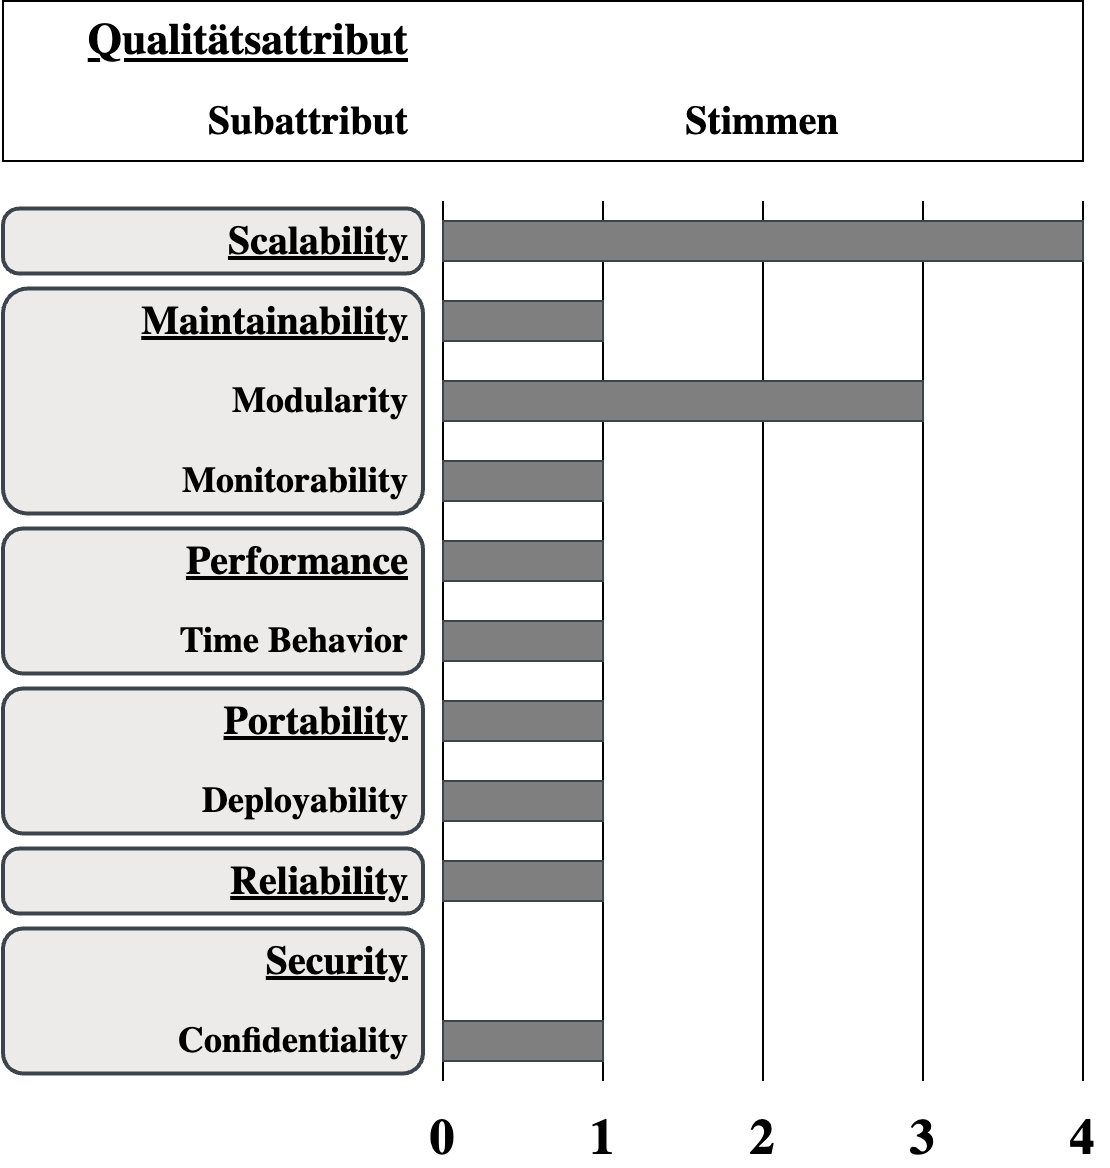
\includegraphics[width=0.6\textwidth]{qas-priority.drawio}
	\caption[Umfrageergebnisse wichtigste (Sub-) QAs im Architekturreview]{
		Umfrageergebnisse bei der Suche nach den wichtigsten (Sub-) QAs im Ar\-chi\-tek\-tur\-review in Phase 1 der Migration mit N = 5.
	}
	\label{fig:qas-priority}
\end{figure}
Dabei ist auffällig, dass auch  \acrlongpl{qa} Stimmen erhalten haben.
Das liegt daran, dass nicht alle Teilnehmer der Umfrage sich auf Sub-\glspl{qa} beschränkt haben, sondern auch die \glspl{qa} \emph{Performance}, \emph{Reliability}, \emph{Maintainability} und \emph{Portability} genannt wurden.
Auch wenn das nicht so vorgesehen war, wurde davon abgesehen, die Teilnehmer darauf hinzuweisen und es zu korrigieren, da die Ergebnisse nicht direkt zur Priorisierung der Attribute führen müssen.
Stattdessen wurden die Umfrageergebnisse und als vage Basis für eine freiere Diskussion über die Priorisierung verwendet.
Deren Ergebnis war die schlussendliche Platzierung der sechs wichtigsten Sub-\glspl{qa}.
Im Folgenden werden diese erläutert.
\begin{enumerate}
	\item \textbf{\emph{Scalability}} ist ein \gls{qa} ohne Subattribute, es wird allerdings auch oft \emph{Performance} zugeordnet. Nach \Citet{master-daniel-koch} gibt es an, wie effizient ein System skaliert werden kann~\cite{koch-scalability-1}. Im Kontext von Microservices ist dabei vor allem die horizontale Skalierung relevant, welche die Skalierung über mehrere Instanzen von der Microservices beschreibt~\cite{koch-scalability-2}.
	\item \textbf{\emph{Modularity}} ist ein Subattribut von \emph{Maintainability}. Nach \Citet{master-daniel-koch} gibt es an, wie gut die Komplexität des Systems auf verschiedene Komponenten verteilt ist~\cite{ISO-25010}.
	\item \textbf{\emph{Time Behavior}} ist Subattribut von \emph{Performance}. Nach \Citet{master-daniel-koch} gibt es an, wie schnell ein System oder Teile eines Systems ankommende Anfragen beantworten~\cite{ISO-25010,koch-time-behavior-1,koch-time-behavior-2}.
	\item \textbf{\emph{Deployability}} ist ein Subattribut von \emph{Portability}. Nach \Citet{master-daniel-koch} gibt es an, wie einfach und schnell ein Produkt gebaut und ausgeliefert werden kann~\cite{koch-scalability-1,koch-deployability}.
	\item \textbf{\emph{Fault Tolerance}} ist Subattribut von \emph{Reliability}. Nach \Citet{master-daniel-koch} gibt es an, inwieweit ein System wie erwartet funktionieren kann, obwohl in Teilen des Systems Fehler auf\-tre\-ten~\cite{ISO-25010,koch-fault-tolerance}.
	\item \textbf{\emph{Recoverability}} ist ebefalls Subattribut von \emph{Reliability}. Nach \Citet{master-daniel-koch} gibt es an, inwieweit ein System nach einem Ausfall wieder den Zustand vor dem Ausfall herstellen kann, sowie Daten erhalten kann~\cite{ISO-25010}.
\end{enumerate}
Die genaue Anzahl der wichtigsten (Sub-)Attribute war nicht vor dem Termin definiert, sondern wurde ebenfalls von der Gruppe diskutiert (in einem späteren Schritt) und gemeinsam auf sechs festgelegt.
Der gesamte Prozess der Umfrage und anschließender Diskussion, um die Prioritäten der Attribute zu setzen, dauerte etwa 15 Minuten und entsprach somit der geplanten Zeit.

\subsection{Szenarienerhebung (Schritt 3)}

Im nächsten Schritt war die Aufgabe, für jedes dieser (Sub-) \glspl{qa} zwei Szenarien zu definieren, die das Attribut gut und auf verschiedene Arten beschreiben.
Es wurde keine spezielle Methodik an\-ge\-wandt, sondern in einer offenen Diskussion der gesamten Gruppe von verschiedenen Teil\-neh\-mern nacheinander für die Attribute Szenarien vorgeschlagen und anschließend überarbeitet oder teilweise auch abgelehnt.
Diese Szenarien wurden in Form eines \emph{Utility Trees}, beschrieben in \cref{sec:atam-saam-svahnberg}, festgehalten.
Nach einer Diskussionszeit von etwa 35 Minuten ergaben sich die Szenarien, die in  \cref{fig:scenarios} abgebildet sind.

\begin{figure}
	\centering
	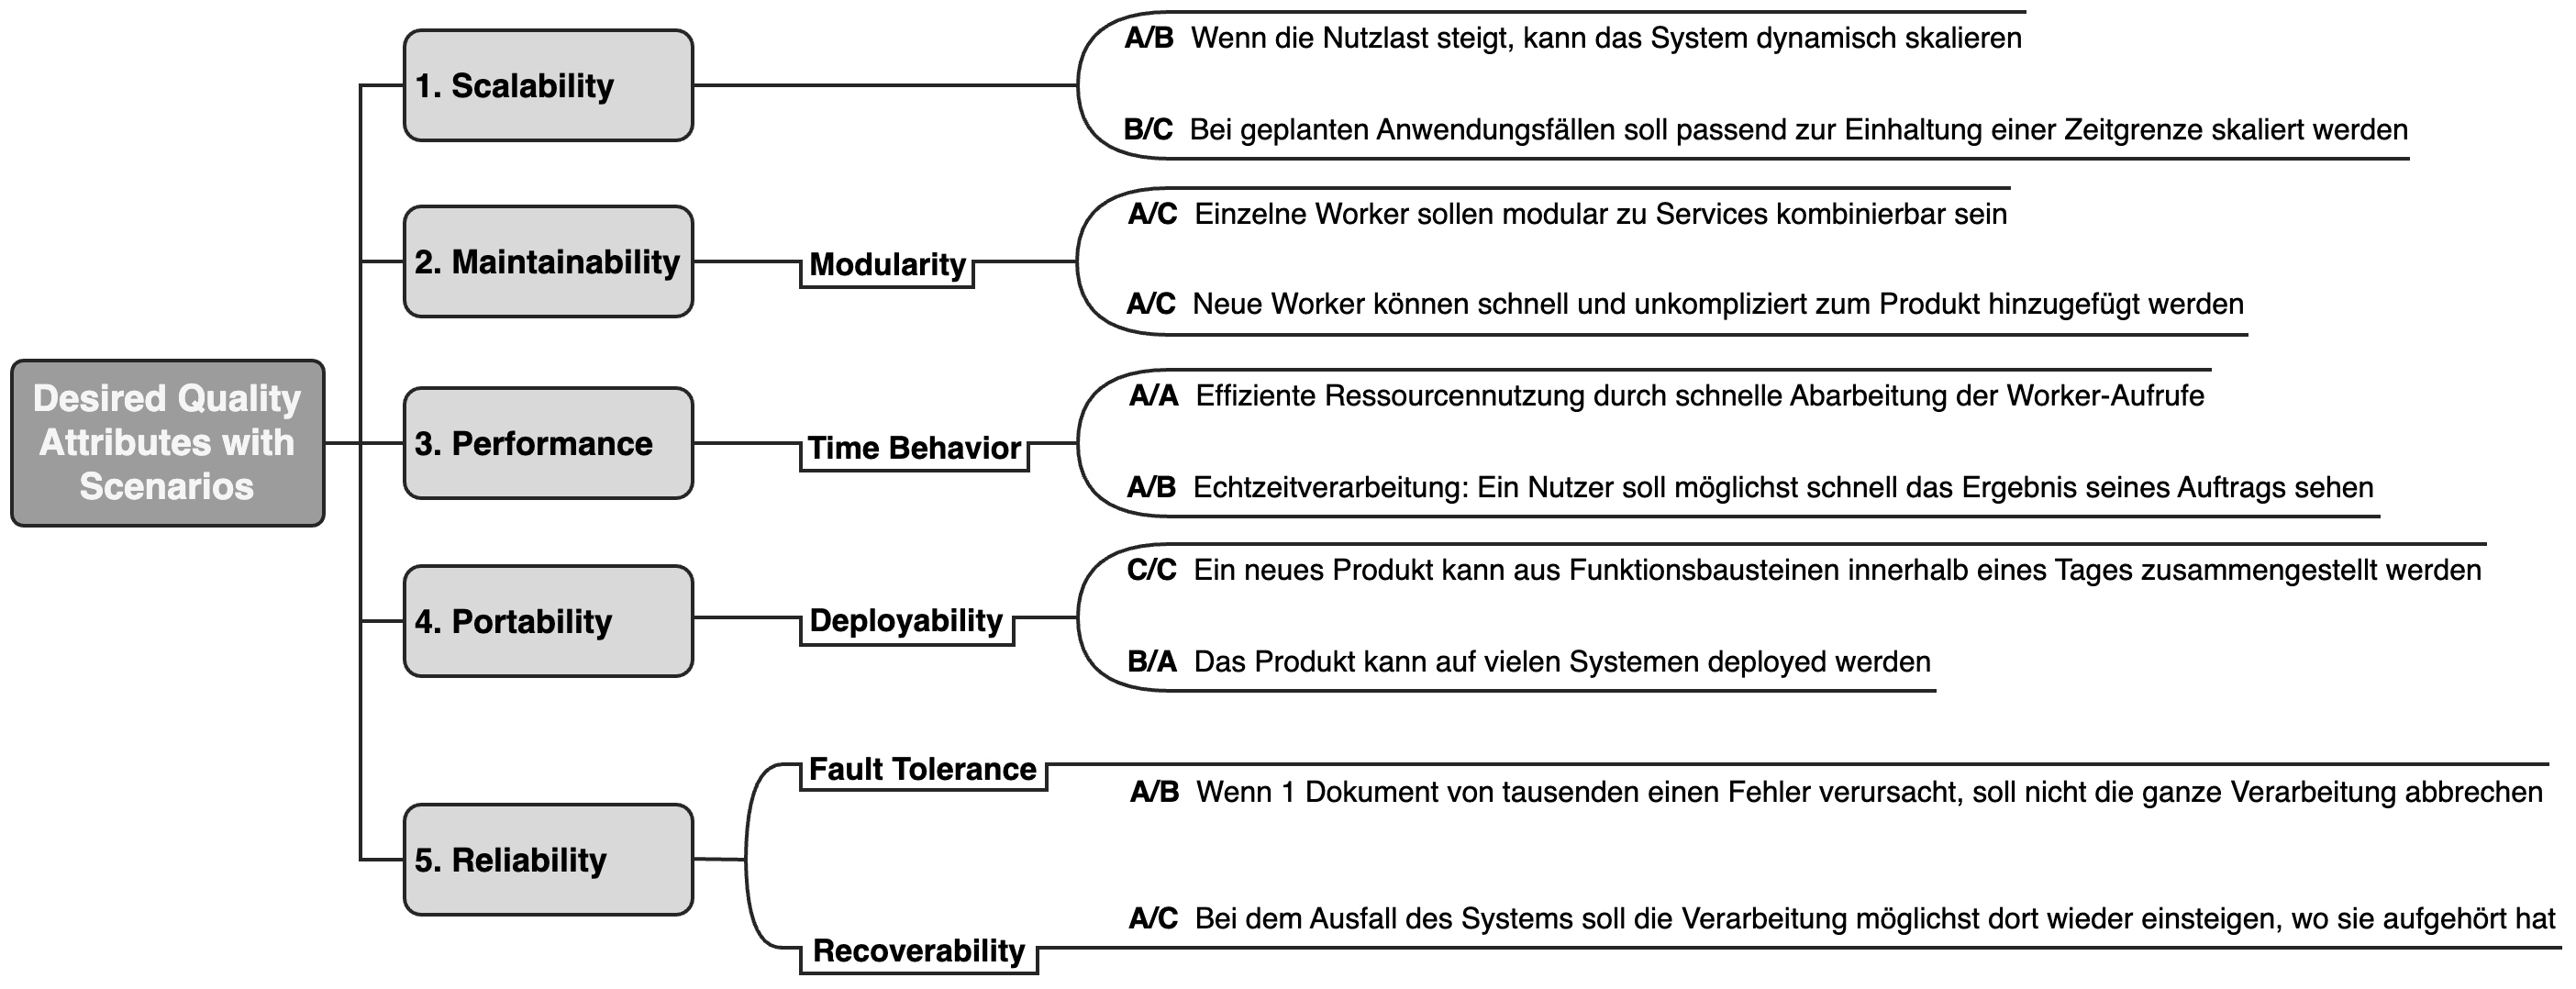
\includegraphics[angle=270,width=\textwidth]{scenarios.drawio}
	\caption[Utility Tree des Architekturreviews mit \acrshortpl{qa} und Szenarien]{
		Der Utility Tree mit Szenarien, die aus dem in Phase 1 durchgeführten Architekturreview resultieren.
		Von oben nach unten enthält der Baum folgende Elementarten: [1] Wurzel (ohne Bedeutung), [2] \gls{qa}, [3] Subattribut, [4] Be\-ur\-teilung des Szenarios hinsichtlich Wichtigkeit und technischer Schwierigkeit, [5] Szenariobeschreibung.
	}
	\label{fig:scenarios}
\end{figure}

Wie aus der Abbildung ersichtlich, wurden für jedes (Sub-)Attribut mit Ausnahme von \emph{Fault Tolerance} und \emph{Recoverability} jeweils zwei Szenarien erstellt.
Dies hat zwei Gründe.
Zum einen wurden für diese Subattribute keine ausreichend unterschiedlichen Szenarien gefunden.
Zum anderen wurde in diesem Fall ein Szenario als ausreichend betrachtet, da Reliability das einzige QA ist, für das mehrere Subattribute eingeschlossen wurden.
Darüber hinaus ist es das am geringsten priorisierte Attribut.

Um zusätzliche eine Priorisierung der Szenarien vornehmen zu können, sieht der \gls{arh} jeweils eine dreistufige Bewertung der Szenarien hinsichtlich ihrer Wichtigkeit und ihrer technischen Schwierigkeit vor.
Diese wurde im nächsten Schritt vorgenommen.
Dabei haben die Teilnehmer die Szenarien der Reihe nach betrachtet und die genannten Eigenschaften diskutiert.
Nicht immer waren alle anfangs einer Meinung, doch schlussendlich konnte nach etwa 35 Minuten für jedes Szenario Konsens gefunden und dieser Schritt abgeschlossen werden.

Da die Vollendung des dritten Schritts nach \Citet{SVAHNBERG20071893} länger gedauert hat als geplant, waren am Ende dieses Termins nur noch wenige Minuten übrig.
Für alle Sub-Schritte dieses Schritts zusammen waren nur 60 Minuten eingeplant, das Sammeln der Szenarien und das Bewerten dieser (also zwei von drei Sub-Schritten) nahm jedoch schon 70 Minuten in Anspruch.
Daher wurde entschieden, die restlichen Punkte in einer weiteren Sitzung in der nächsten Woche zu bearbeiten.

Am 14. November 2023 wurde dann der zweite Teil des Architekturreviews durchgeführt.
Anwesend waren dieselben Personen.
Da bei diesem Treffen ein neuer Blickwinkel auf die Thematik möglich gewesen wäre, wurden zunächst zehn Minuten darauf verwendet, die bereits vorhandenen Szenarien und die Bewertung dieser hinsichtlich Wichtigkeit oder technischer Schwierigkeit erneut zu überprüfen und Raum für mögliche Änderungen zu schaffen.
Es wurden jedoch keine Änderungen vorgenommen und die Teilnehmer bestätigten lediglich erneut die bereits vorhandenen Szenarien.

Anschließend wurde wie geplant damit fortgefahren, den Szenarien weitere \glspl{qa} zuzuordnen.
Oft können trotz der Erstellung eines Szenarios für ein bestimmtes \gls{qa} weitere \glspl{qa} damit assoziiert werden.
Deswegen wurde erneut jedes Szenario betrachtet und diskutiert, welche weiteren (Sub-) Attribute darauf zutreffen könnten.
Nach etwa 15 Minuten Diskussion waren alle Szenarien behandelt und für jedes einstimmig geklärt, welche weiteren Subattribute damit assoziiert werden.
Diese werden folgend im Bezug auf die jeweiligen Szenarios sekundäre \glspl{qa} genannt, wohingegen ein \gls{qa}, für das das Szenario erstellt wurde, primäres \gls{qa} genannt wird.
Die resultierenden Assoziationen sind in der \cref{tab:scenarios} aufgeführt.

\begin{table}[!h]
  \centering
  \begin{tabular}{ m{2,3cm} m{6cm} m{0.7cm} m{2,5cm} p{0.7cm} }
    \toprule
    \textbf{Name} & \textbf{Beschreibung} & \textbf{W/S} & \textbf{\glspl{qa}} & \textbf{MS} \\
    \midrule
    Dynamische Ska\-lier\-bar\-keit & Wenn die Nutzlast steigt, kann das Sys\-tem dynamisch skalieren & A/B & Scalability, Re\-source Uti\-li\-za\-tion, Adaptability, Execution Cost & \advantage \\ \hline
    Statische Ska\-lier\-bar\-keit & Bei geplanten Anwendungsfällen soll passend zur Einhaltung einer Zeitgrenze skaliert werden & B/C & Scalability, Resource Utilization, Time Behavior & \advantage \\  \hline
    Jobtemplates& Einzelne Worker sollen modular zu Services kombinierbar sein & A/C & Modularity, Reusability & - \\ \hline
    Neue Worker& Neue Worker können schnell und un\-kom\-pliziert zum Produkt hinzugefügt werden & A/C & Modularity, Reusability & \advantage  \\ \hline
    Schnelle Ab\-ar\-bei\-tung & Effiziente Ressourcennutzung durch schnelle Abarbeitung der Worker-Auf\-rufe  & A/A & Time Behavior, Resource Uti\-li\-za\-tion & \disadvantage \\ \hline
    \glqq Echtzeit\grqq{}-Verarbeitung & Ein Nutzer soll möglichst schnell das Ergebnis seines Auftrags sehen & A/B & Time Behavior & \disadvantage \\ \hline
    Einfaches De\-ploy\-ment & Ein neues Produkt kann aus Funk\-tions\-bausteinen innerhalb eines Tages zusammengestellt werden &C/C & Deployability, Modularity, Agility & \disadvantage \\ \hline
    Platform-unabhängigkeit& Das Produkt kann auf vielen Systemen deployed werden & B/A & Deployability, Installability & \advantage \\ \hline
    Fehlerto\-leranz Massen\-ver\-ar\-beitung & Wenn 1 Dokument von tausenden einen Fehler verursacht, soll nicht die ganze Verarbeitung abbrechen & A/B & Fault-Tolerance &\advantage \\ \hline
    Erholen nach Sys\-tem\-ausfall & Bei dem Ausfall des Systems soll die Verarbeitung möglichst dort wieder einsteigen, wo sie aufgehört hat & A/C & Recoverability & - \\
    \bottomrule
  \end{tabular}
  \caption[Im Architekturreview ermittelte Qualitätsanforderungen und Szenarien]{
    Szenarien, die aus dem in Phase 1 durchgeführten Architekturreview resultieren.
    \emph{W/S} gibt die Wichtigkeit/Schwierigkeit der Szenarien in drei Stufen an (A steht für sehr wichtig und sehr schwierig).
    \emph{\glspl{qa}} gibt die Assoziation der Szenarien zu bestimmten \acrfullpl{qa} an; zuerst genannte sind primäre \glspl{qa}, folgende sekundäre \glspl{qa}.
    \emph{MS} gibt die Einschätzung darüber an, ob das jeweilige Szenario von einer Microservices-Architektur profitiert.
  }
  \label{tab:scenarios}
\end{table}


Damit wurde der für die Extraktion der Qualitätsanforderungen des Systems relevante Teil des Architekturreviews abgeschlossen.
Zusammenfassend kann gesagt werden, dass die Phase größtenteils wie geplant durchgeführt werden konnte.
An einigen Stellen sind die verschiedene Schritte etwas verschmolzen oder es wurde kurz zu vorherigen Schritten zurückgesprungen, was jedoch vollkommen normal ist und auch beispielsweise in \gls{atam} von \Citet{kazman_2000} als gängige Praxis beschrieben wird.
So wurde in diesem Fall beim Erstellen der Szenarien entschieden, bis zu welcher Priorität die \glspl{qa} mit Szenarien versehen werden, obwohl die Wahl der Anzahl der wichtigsten tatsächlich für den vorherigen Schritt geplant war.
Die Beteiligung der Teilnehmer war nicht komplett ausgeglichen, aber jeder hat regelmäßig etwas beigetragen.
Es kann angenommen werden, dass das Ergebnis von allen Teilnehmern ausreichend geformt wurde und dass keine einseitige Beeinflussung vorliegt.

\subsection{Architekturanalyse anhand Szenarien (Schritt 5)}

Neben der Erfassung der wichtigsten Szenarien und \glspl{qa} hatte die Fokusgruppe als sekundäres Ziel, die Wahl der Architektur für \emph{jadice flow} zu bewerten.
Diese Bewertung wurde ebenfalls in der zweiten Sitzung des Architekturreviews durchgeführt und entspricht dem vierten Schritt \emph{Assessment} der ersten Phase des \gls{arh}.
Da dieser Schritt jedoch noch nicht im Tool implementiert ist, wurde er manuell durchgeführt.
Im Gegensatz zu vorherigen Schritten der ersten Phase ist dieser nicht relevant für die nächsten Phasen, weshalb es kein Problem ist, den \gls{arh} hierbei nicht zu verwenden.
In diesem Schritt wurde die Frage diskutiert, ob eine \acrlong{msa} individuell für jedes Szenario vorteilhaft ist im Vergleich zu einer monolithischen Architektur.
Hierbei wurde in drei Stufen unterschieden:
\begin{itemize}
	\item \advantage\hspace*{0.1cm}: Dieses Szenario profitiert wesentlich mehr von einer \gls{msa} als von einer monolithischen Architektur.
	\item \disadvantage\hspace*{0.1cm}: Dieses Szenario profitiert wesentlich mehr von einer monolithischen Architektur als von einer \gls{msa}.
	\item \hspace*{0.27cm}-\hspace*{0.27cm}: Dieses Szenario profitiert in verschiedenen Punkten sowohl von einer \gls{msa} als auch von einer monolithischen Architektur, wobei sich beide Seiten ungefähr gleichen.
\end{itemize}
Bei Szenarios wie beispielsweise den des \emph{Scalability} Attributs war es nicht schwer, Konsens zu finden, da die Möglichkeit der Skalierung auf Service-Ebene einer der größten Vorteile von \glspl{msa} gegenüber Monolithen ist.
In anderen Fällen jedoch war es schwieriger, abzuwägen, ob die Vorteile einer \gls{msa} oder die eines Monolithen überwiegen.
Schlussendlich konnte jedoch in Form von offener  Diskussion für jedes Szenario einstimmig geklärt werden, welche der drei Optionen gewählt werden sollte, sodass keine Abstimmungen notwendig waren.

Das Ergebnis dieser Einschätzungen ist ebenfalls in \cref{tab:scenarios} zu sehen.
Insgesamt wurde eine \gls{msa} in fünf Fällen als vorteilhaft und nur in drei Fällen als unvorteilhaft bewertet.
Des Weiteren ist zu beachten, dass die Szenarien in der Tabelle nach der Wichtigkeit der primären \glspl{qa} sortiert sind und die obersten beiden Szenarien die Hauptfaktoren für die Migration zu einer Microservices-Architektur waren.
Durch die Überlegenheit der \gls{msa}-Favorisierungen und dass diese verstärkt bei den höchst priorisierten \glspl{qa} (siehe \cref{tab:scenarios}) vorliegen, kann diese Auswertung die Entscheidung zur Migration zu einer \gls{msa} bestätigen.

Nachdem nun erwünschte Szenarien und \glspl{qa} erhoben wurden und die Wahl einer \gls{msa} für \emph{jadice flow} bekräftigt wurde, kann mit Phase 2 fortgefahren werden.

\section{Phase 2 - Strategieplanung}
\label{sec:durchführung-phase2}

In dieser Phase wird die Suchfunktion des \gls{arh} verwendet, um geeignete Migrationsstrategien zu finden.
Diese Suche wird dabei von zwei Faktoren beeinflusst: dem Ergebnis der Phase 1 in Form von \glspl{qa} beziehungsweise Szenarien und zusätzlichen Filtern, die vor der Suche konfiguriert werden müssen.
Im Folgenden werden diese Filter in konfiguriert, mehrere Suchen mit ihnen und den \glspl{qa} aus Phase 1 definiert, durchgeführt und dann aggregiert.
Abschließend werden die Ergebnisse dessen analysiert.

\subsection{Filterselektion}
\label{sec:filterselektion}

Um möglichst passende Ergebnisse bei der Suche nach Migrationsmethoden zu erhalten, die den Vorstellungen der Architekten und dem Zielsystem entsprechen, bietet der \gls{arh} neben der Konfiguration der Szenarien weitere Filtermöglichkeiten.
In diesem Abschnitt werden Filter aus einer Auswahl von insgesamt  71 verschiedenen Filtern aus fünf Kategorien und 16 Unterkategorien ausgewählt.
Für jede der Eigenschaften aus \cref{tab:phase2-all-filter} kann eine der folgenden drei Präferenzen angegeben werden:
\begin{itemize}
	\item \textbf{Include:} Methoden, die die jeweilige Eigenschaft besitzen, werden höher platziert.
	\item \textbf{Neutral:} Ob Methoden die jeweilige Eigenschaft besitzen oder nicht, wirkt sich nicht auf ihre Platzierung aus.
	\item \textbf{Exclude:} Methoden, die die jeweilige Eigenschaft nicht besitzen, werden höher platziert.
\end{itemize}

\begin{table}%[!h]
  \centering
  \begin{tabular}{m{2cm} m{2cm} m{9cm}}
    \toprule
    \textbf{Kategorie} & \textbf{Subkategorie} & \textbf{Filter} \\
    \midrule
    Quality Preferences & System Properties & \prioOne{Autonomy}, Cohesion, \prioTwo{Complexity}, Coupling, \prioOne{Granularity}, \prioTwo{Isolation},  \prioOne{Technology Heterogenity} \\ \hline
    \multirow{4}{=}[-1cm]{Input Preferences} & Domain Artifacts &  Documentation,  \prioOne{Human Expertise}, Ontology, \prioTwo{Version Control System} \\ \cline{2-3}
    & Runtime Artifacts &  \prioTwo{Log Traces}, User-Application Interactions \\ \cline{2-3}
    & Model artifacts & Activity diagram, Business Process Model, Class diagram, Custom model, Data Flow Diagram, Entity Model, State Machine Diagram, Use Case Model \\ \cline{2-3}
    & Executables &  \prioOne{API / Interface}, Database File,  \prioTwo{Source Code (Java)},  \prioOne{Source Code (No Specification)}, Source Code (Python), Test Cases \\ \hline
    \multirow{6}{=}[-1.9cm]{Process Preferences} & Directions & Bottom-Up, Mixed, Top-Down \\ \cline{2-3}
    & Levels of Automation & Automatic, Manual, Semi-Automatic \\ \cline{2-3}
    & Analysis Types & Dynamic, Historic, Lexical, Static \\ \cline{2-3}
    & Techniques & Clustering, Custom Heuristics, Data-Flow Driven, Domain-Driven Design, Execution-Trace Modeling, General Guidelines, Genetic Algorithm, Graph-based, Machine Learning, Multi-Tenancy, Performance Modeling, Scenario Analysis, Wrapping / Black Box \\ \cline{2-3}
    & Process Strategy & Continuous Evolution, Extension, Greenfield,  \prioOne{Refactor}, Rewrite / Rebuild, Strangler \\ \cline{2-3}
    & Atomar Unit & Business Capability, Class, Entity, Function, Functionality, Interface, Other \\ \hline
    Output Preferences & Representation &  \prioTwo{Guideline / Workflow},  \prioOne{List of services}, Source Code,  \prioOne{Splitting recommendations}, Visualization \\ \hline
    \multirow{4}{=}[-1cm]{Usability Preferences} &Validation Methods & Case Study, Experiment, Industry, No Validation \\ \cline{2-3}
    & Accuracy of \gls{sia} & High, Medium, Low, Not Available \\ \cline{2-3}
    & Tool Support & No Tool Support \\ \cline{2-3}
    & Tool Types & Database, Decomposition, Dynamic Analysis, Java, Open Source, Other, Reverse Engineering, Static Analysis, Visualization \\
    \bottomrule
  \end{tabular}
  \caption[Mögliche Filter des \gls{arh} in Phase 2]{
  	Mögliche Filter des \gls{arh} in Phase 2 bei der Suche nach Migrationsstrategien.
  	Die in dieser Thesis verwendeten Filter (mit \emph{include}) sind folgendermaßen markiert:
    \prioTwo{Unterstrichene Filter} sind Filter mit geringerer Priorität (Priorität 2, insgesamt sechs Filter).
    \prioOne{Unterstrichene und fett markierte Filter} sind Filter mit hoher Priorität (Priorität 1, insgesamt neun Filter).
  }
  \label{tab:phase2-all-filter}
\end{table}


Die Entwickler des \gls{arh} empfehlen, präferierte Eigenschaften auf \emph{include} zu setzen und die anderen auf der Standardeinstellung \emph{neutral} zu belassen und die Einstellung \emph{exclude} nur selten zu verwenden, da der Ausschluss einer Eigenschaft typischerweise nicht das Ziel ist.
Wenn eine Eigenschaft nicht erwünscht ist, kann es in vielen Fällen möglich sein, die Methode minimal abzuändern oder einen Teil der Methode zu ignorieren.
Dadurch sollte eine solche unerwünschte Eigenschaft trotzdem kein Problem darstellen und die Methode nicht schlechter bewertet werden.

Für die Wahl der Filter für das Refactoring von \emph{jadice flow} wurden alle Filter gemeinsam von Autor und \gls{po} betrachtet und dabei evaluiert, welche am besten auf diesen Fall zutreffen (\cref{feldnotiz:1,feldnotiz:2}).
\emph{Ausgewählt} bedeutet in diesem Kontext, dass der entsprechende Filter auf \emph{include} gesetzt wurde.
Die Option \emph{exclude} wurde nicht verwendet.
Dabei wurden die ausgewählten Filter in zwei Prioritätsstufen unterteilt (\cref{feldnotiz:3}).
Filter mit Priorität 1 sind dabei die höher priorisierten Filter.
Diese bilden die realistische Auswahl an Filtern ab, die verwendet worden wären, wenn nur ein Suchdurchgang durchgeführt werden würde.
Diese Unterteilung in mehrere Prioritätsstufen ist dazu konzipiert, Suchvorgänge mit verschiedenen Filterkonfigurationen durchführen zu können, um mehrere mögliche Anwendungsfälle zu testen.
Eine ausführlichere Beschreibung dazu ist in \cref{sec:phase2-suchconfig} gegeben.
Die ausgewählten Filter sind in \cref{tab:phase2-all-filter} markiert und in \cref{tab:phase2-selected-filter} einzeln aufgelistet.

\begin{table}[!h]
  \centering
  \begin{tabular}{m{3cm} l m{4cm} m{3.5cm}}
    \toprule
    \textbf{Kategorie} & \textbf{Subkategorie} & \textbf{Filter Priorität 1} & \textbf{Filter Priorität 2} \\ \midrule
    Quality Preferences & System Properties & Autonomy, Granularity, Tech\-nology Heterogenity & Complexity, Isolation \\ \hline
%    \multirow{3}{=}[-0.3cm]{Input Preferences} In die mittlere Zeile schreiben sollte es besser zentrieren
    & Domain Artifacts & Human Expertise & Version Control Sys\-tem \\
    Input Preferences & Runtime Artifacts & - & Log Traces \\
     & Executables & API/Interface, Source Code (No specifica\-tion) & Source Code (Java) \\ \hline
    Process Preferences & Process Strategy & Refactor & - \\ \hline
    Output Preferences & Representation & List of services, Split\-ting recommendations & Guideline/ Workflow \\ \hline
    Usability Preferences & - & - & - \\ \midrule
    \multicolumn{2}{l}{\textbf{Summe}} &\textbf{9} & \textbf{6} \\ \bottomrule
  \end{tabular}
  \caption[Gewählte Filter des \acrshort{arh}]{
    Gewählte Filter des \gls{arh} in Phase 2 bei der Suche nach Migrationsstrategien.
    Unterteilt in zwei Prioritätsstufen, wobei Filter der Priorität 1 in einer Evaluationsrunde von Autor und \gls{po} als wichtiger eingestuft wurden.
%    Filter mit Priorität 2 werden nur bei der Suche mit allen Filtern verwendet.
%    Mit 1 priorisierte Filter werden sowohl bei der Suche mit allen als auch in der Suche mit den wichtigsten Filtern verwendet.
  }
  \label{tab:phase2-selected-filter}
\end{table}


Bei der Auswahl der Filter, die vom Autor und \gls{po} durchgeführt wurde, haben die folgenden Begründungen zur schlussendlichen Filterwahl geführt:
Allgemein wurde darauf geachtet, nur die notwendigsten Filter auszuwählen, um den Einfluss einzelner Filter nicht zu verringern.
Als gewünschte Zieleigenschaften des Systems wurden die \glspl{sp} als besonders wichtig erachtet.
Daher wurden insgesamt fünf von sieben verfügbaren Filtern aus dieser Kategorie aufgenommen.
Neben den Filtern dieser Kategorie wurden vor allem die Filter der Kategorien \emph{Input Preferences} und \emph{Output Preferences} betrachtet.
Diese hängen ebenfalls stark vom System ab und betreffen die Ausgangslage sowie das gewünschte Ergebnis.
Deshalb wurden insgesamt sechs Filter aus der Kategorie \emph{Input Preferences} und vier aus der Kategorie \emph{Output Preferences} gewählt.
Andere Kategorien, wie \emph{Process Preferences} und \emph{Usability Preferences}, welche die interne Funktionsweise der Methode betreffen, wurden als unwichtiger und vor allem unabhängiger vom betreffenden System eingestuft.
Als einziger Filter in diesen Kategorien wurde bei der Prozess-Strategie die Eigenschaft \emph{Refactoring} gewählt.
Da bereits eine \gls{msa} vorliegt wären die anderen Optionen wie \emph{Rewrite/Rebuild} in diesem Fall wenig sinnvoll.

\subsection{Konfiguration der Suchen}
\label{sec:phase2-suchconfig}

Die im vorherigen Abschnitt gewählten und in zwei Prioritäten unterteilten Filter werden nun verwendet, um mehrere Suchdurchgänge zu definieren.
Das Ziel des Einsatzes mehrerer Suchen mit jeweils unterschiedlichen Eingaben besteht darin, die Filter- und Suchfunktion anhand der unterschiedlichen Ergebnisse zu evaluieren.
Um mehrere Suchen zu definieren, wurde die Konfiguration ausgehend von der realistischen Suchkonfiguration, die folgend \emph{Wichtigste Filter} genannt wird, variiert.
Realistisch bedeutet dabei, dass diese Konfiguration verwendet worden wäre, wenn nur eine Suche durchgeführt worden wäre.

Wie in \cref{tab:phase2-search-description} in der zweiten Spalte dargestellt, beinhaltet diese \emph{wichtigste Suche} alle \glspl{qa} und die Filter der Priorität 1.
Ausgehend davon wurde für die weiteren Suchkonfigurationen in zwei Dimensionen variiert.
In der ersten wurden die \glspl{qa} gleich belassen und die Filter variiert (Spalten 2 und 3 der \cref{tab:phase2-search-description}).
In der zweiten Dimension wurden ausgehend von der realistischen Eingabe der Filter (höchst priorisierte Filter) die \glspl{qa} variiert.
Da die Anzahl der Szenarien mit zehn als relativ hoch eingeschätzt wurde und das Erschließen neuer Szenarien ein erneutes Architekturreview benötigt hätte, wurde vom Autor beschlossen, in dieser Dimension lediglich eine Reduktion der Anzahl der Szenarien durchzuführen.
Das Entfernen von bis zu 4 Szenarien ergab hierbei keine veränderten Ergebnisse, weswegen in dieser Dimension nur eine zusätzliche Suche komplett ohne \glspl{qa} aufgeführt wird.
Dadurch soll die Zahl der Suchen begrenzt werden.

%Um eine begrenzte Auswahl der Verfahren für die detaillierte Betrachtung sicherzustellen, wurden folgende Schritte unternommen:
%Es wurden vier Suchen mit verschiedenen Konfigurationen der Filter und \glspl{qa} (Übersicht in \cref{tab:phase2-search-description}) durchgeführt.
%Dabei wurde ausgehend von der realistischsten Eingabe in zwei Di\-men\-sio\-nen variiert: die der Filter und die der \glspl{qa}.
%Die realistischste Eingabe ist die Verwendung aller \glspl{qa} und der wichtigsten Filter.
%In der ersten Dimension wurden ausgehend davon die Filter variiert.
%Es wurde zusätzlich eine Suche mit allen Filtern und eine ohne Filter durchgeführt.
%In der zweiten Dimension wurden ausgehend von der realistischen Eingabe der Filter (höchst priorisierte Filter) die \glspl{qa} variiert.
%Da das Entfernen von bis zu 4 Szenarien keine anderen Ergebnisse ergab, wird in dieser Dimension nur eine zusätzliche Suche komplett ohne \glspl{qa} aufgeführt, um die Ergebnisse übersichtlicher zu halten.
%Die Verwendung mehrerer Suchen soll einerseits zu besseren Ergebnissen führen und andererseits die Suchfunktion auf Basis der Filter und \glspl{qa} untersuchen.

\begin{table}[!ht]
	\centering
	\begin{tabular}{|c| c | c c | c|}
	\toprule
	\multirow{2}{*}[0cm]{\textbf{\diagbox{Filter}{Suche}}} & \textbf{Wichtigste Filter} & \textbf{Alle Filter} & \textbf{Keine Filter} & \textbf{Keine \glspl{qa}} \\
	& Realistischste Eingabe & \multicolumn{2}{c|}{Dimension Filter} & Dimension \glspl{qa} \\ \midrule
	\textbf{\glspl{qa}} (17) & Inkl.  & Inkl. & Inkl. & Exkl. \\
	\textbf{Filter Priorität 1} (9) & Inkl. & Inkl. & Exkl. & Inkl. \\
	\textbf{Filter Priorität 2} (15) & Exkl. & Inkl. & Exkl. & Exkl. \\ \bottomrule
	\end{tabular}
	\caption[Suchkonfigurationen für die Suchen nach Migrationsverfahren]{
    Konfigurationen der verschiedenen Suchen nach Migrationsverfahren in Phase 2 des \gls{mmf}.
    Die Zeilen beschreiben verschiedene Teilmengen der Filter und \glspl{qa}.
    In den Spalten sind die Konfigurationen der vier Suchen zu sehen und welche der Teilmengen sie inkludieren (inkl.) oder exkludieren (exkl.).
    In Klammern hinter den Überschriften ist dargestellt, wie viele Filter die Teilmengen beinhalten.
  }
	\label{tab:phase2-search-description}
\end{table}


\subsection{Selektions- und Aggregationsstrategie}
\label{sec:phase2-suchaggregation}

Bei Anwendung der im vorherigen Abschnitt definierten Suchen werden sich vier Listen von Er\-gebnissen ergeben.
Um ein strukturiertes Vorgehen bei der Auswahl der Ergebnisse, die manuell betrachtet werden sollen, zu gewährleisten, werden diese Listen vor Betrachtung zu einer Liste aggregiert.
Folgend wird beschrieben, wie diese Aggregation entworfen und durchgeführt wurde.

Um die Auswahl der Ergebnisse, die manuell betrachtet werden sollen, auf eine adäquate Größe einzugrenzen, werden nur die ersten fünf Ergebnisse jeder Suche in die aggregierte Liste übernommen.
Außerdem werden alle dem fünften Ergebnis folgenden Ergebnisse übernommen, die die gleiche Anzahl an Übereinstimmungen aufweisen wie das fünfte.
Dadurch soll die Anzahl an Übereinstimmung als einziges Kriterium für die Ordnung und Auswahl sichergestellt werden, damit andere Faktoren wie eine mögliche lexikalische Ordnung oder Ordnung nach Identifikationsnummer keinen Einfluss erhalten.

Für eine bessere Übersicht über die selektierten Ergebnisse werden diese anschließend geordnet.
Dafür wird die Metrik $m_{gesamt}$ für die Gesamtwertung jedes Verfahrens definiert.
Diese gesamte prozentuale Übereinstimmung jedes Verfahrens $m_{gesamt}$ ist ein gewichtetes arithmetisches Mittel der prozentualen Übereinstimmungen des Verfahrens in jeder der vier Suchen.
Diese sind $m_{Wichtigste \text{ } Filter}$, $m_{Alle \text{ } Filter}$, $m_{Keine \text{ } Filter}$ und $m_{Keine \text{ } \glspl{qa}}$, wobei die Namen sich nach \cref{tab:phase2-search-description} richten und die Werte in der Spalte \emph{Matches, Insgesamt} der \cref{tab:phase2-filter-results} gefunden werden können.
Das wären beispielsweise im Fall \Citet{arh-result-no-filter-1} $m_{Wichtigste \text{ } Filter} = \frac{14}{26} \approx 53,8\%$.

$m_{gesamt}$ wird wie folgt berechnet:
\[
m_{gesamt} = \frac{m_{Wichtigste \text{ } Filter} + 0,75 \cdot  m_{Alle \text{ } Filter} +  0,5 \cdot m_{Keine \text{ } Filter} + 0,25 \cdot m_{Keine \text{ } \glspl{qa}}}{2,5}
\]
Die Gewichtung der verschiedenen Suchen ist so gewählt, dass die realistische Suche das Gewicht 1 hat und die anderen Suchen (mit $0,75$, $0,5$ und $0,25$) weniger stark gewichtet werden.
Damit soll die Relevanz der Suche (eingeschätzt durch den Autor) in die Metrik einfließen.
Für das reine Ordnen der Ergebnisse ist eine Division durch $2,5$ theoretisch nicht nötig.
Um das Ergebnis allerdings eine prozentuale Übereinstimmung nennen zu können, wird durch die Summe der Gewichtungen geteilt.

\subsection{Suchergebnisbetrachtung}

Die Suchen nach Migrationsverfahren wurden wie in \cref{sec:phase2-suchconfig} beschrieben durchgeführt und wie in \cref{sec:phase2-suchaggregation} aggregiert.
Daraus resultieren die Suchergebnisse, die in \cref{tab:phase2-filter-results} dargestellt sind.
\begin{table}%[!ht]
	\centering
	\begin{tabular}{l c c c}
		\toprule
    \textbf{Publikation} & \multicolumn{3}{c}{\textbf{Matches}} \\
     & \textbf{Insgesamt} & \textbf{\gls{qa}} & \textbf{\gls{sp}} \\ \midrule
    \multicolumn{4}{c}{\textbf{Alle Filter (15)}} \\ \midrule
    \Citet{arh-result-no-filter-1} & 15/32 & 11/17 & 0/5 \\ \hline
    \Citet{arh-result-no-filter-3} & 13/32 & 7/17  & 1/5  \\ \hline
    \Citet{arh-result-no-filter-2} & 12/32 & 7/17  & 2/5  \\ \hline
    \Citet{arh-result-no-filter-4} & 11/32 & 7/17  & 0/5  \\ \hline
    \Citet{arh-result-no-filter-5} & 11/32 & 7/17  & 0/5  \\ \midrule
		\multicolumn{4}{c}{\textbf{Wichtigste Filter (9)}} \\ \midrule
		\Citet{arh-result-no-filter-1}        & 14/26 & 11/17 & 0/3 \\ \hline
		\Citet{arh-result-no-filter-3}        & 13/26 & 7/17  & 1/3  \\ \hline
		\Citet{arh-result-no-filter-2}        & 11/26 & 7/17  & 1/3  \\ \hline
		\Citet{arh-result-important-filter-4} & 10/26 & 6/17  & 1/3  \\ \hline
    \Citet{arh-result-no-filter-4}        & 10/26 & 7/17  & 0/3  \\ \hline
    \Citet{arh-result-no-filter-5}      & 10/26 & 7/17  & 0/3  \\ \hline
    \Citet{arh-result-important-filter-7}     & 10/26 & 5/17  & 1/3  \\ \midrule
    \multicolumn{4}{c}{\textbf{Keine Filter (Nur \glspl{qa})}} \\ \midrule
    \Citet{arh-result-no-filter-1} & 11/17 & 11/17 & - \\ \hline
    \Citet{arh-result-no-filter-2} & 7/17  & 7/17  & - \\ \hline
    \Citet{arh-result-no-filter-3} & 7/17  & 7/17  & - \\ \hline
    \Citet{arh-result-no-filter-4} & 7/17  & 7/17  & - \\ \hline
    \Citet{arh-result-no-filter-5} & 7/17  & 7/17  & - \\ \midrule
     \multicolumn{4}{c}{\textbf{Keine \glspl{qa}}} \\ \midrule
     \Citet{arh-result-no-qas} & 8/9  & -  & 3/3 \\ \hline
     \Citet{arh-result-no-filter-3} & 6/9  & -  & 1/3 \\ \bottomrule
	\end{tabular}
	\caption[Surchergebnisse des ARH von Migrationsverfahren mit verschiedenen Filtern]{
		Ergebnisse der Suche mit ARH nach Migrationsverfahren mit verschiedenen Filtern, wie in \cref{sec:filterselektion} näher beschrieben, nach Matches sortiert.
		Insgesamte Matches, \gls{sp} Matches und \gls{qa} Matches entsprechen den im \gls{arh} angezeigten Matches.
	}
	\label{tab:phase2-filter-results}
\end{table}
 % TODO Verschiebung beachten
Die Aggregation der Ergebnisse nach der beschriebenen Aggregations-Metrik ist in \cref{tab:phase2-ranking} zu sehen.
\begin{table}[!h]
  \centering
  \begin{tabular}{l c}
    \toprule
    \textbf{Ergebnis} & \textbf{Matches Prozent ($m_{gesamt}$)} \\ \midrule
    \Citet{arh-result-no-filter-1} & $52\%$ \\ \hline
    \Citet{arh-result-no-filter-3} & $47\%$ \\ \hline
    \Citet{arh-result-no-filter-2} & $41\%$ \\ \hline
    \Citet{arh-result-no-filter-4} & $37\%$ \\ \hline
    \Citet{arh-result-no-filter-5} & $37\%$ \\ \hline
    \Citet{arh-result-important-filter-4} & $36\%$ \\ \hline
    \Citet{arh-result-important-filter-7} & $36\%$ \\ \hline
    \Citet{arh-result-no-qas} & $32\%$ \\
    \bottomrule
  \end{tabular}
  \caption[Prozentuale Übereinstimmung der Suchergebnisse in Phase 2 des \gls{mmf}]{
   	Prozentuale Übereinstimmung der Suchergebnisse in Phase 2 des \gls{mmf}.
  }
  \label{tab:phase2-ranking}
\end{table}
Dabei wurde eine Ausnahme im Bezug auf die beschriebene Selektions- und Aggregationsstrategie bei der Suche ohne \glspl{qa} gemacht.
Bei dieser Suche folgten dem dritten Ergebnis zwölf weitere Ergebnisse mit derselben Punktzahl.
Um die Zahl der Ergebnisse nicht unnötig zu vergrößern wurde hierbei eine Ausnahme gemacht und nur die ersten beiden Ergebnisse übernommen.
Da die Suche in dieser Form experimentell ist und durch das Fehlen von \glspl{qa} nur geringe Relevanz hat, wird darin keine Gefahr für die Validität der Ergebnisse gesehen.

In der Reihenfolge werden die einzelnen Methoden im Folgenden kurz zusammengefasst und anschließend ihre Anwendbarkeit verglichen.

\subsubsection{Ergebnis 1: \citetitle{arh-result-no-filter-1}  \cite{arh-result-no-filter-1}}
\label{sec:phase2-result-1}
\label[res]{res:1}

In dieser Arbeit stellen \citeauthor{arh-result-no-filter-1} ein konzeptuelles Evolutions-Framework vor, das mithilfe von Trans\-for\-ma\-tions\-re\-geln die Migration von Legacy-Systemen zu Microservices unterstützen soll.
Das Vorgehen ist in drei Teilabschnitte unterteilt.

\paragraph{Funktionsweise:} Das \emph{Core System} besteht aus dem Legacy System und einer Auswahl von Transformationsregeln.
Diese können aus der Sammlung der vorgestellten Regeln der Autoren stammen, aber auch durch eigene ergänzt werden.
Daraus wird ein \emph{Middle Layer} erstellt, indem diese Transformationsregeln auf das Legacy-System angewendet werden.
Das Resultat dessen ist eine Dekomposition des Systems in Microservices.
Das \emph{Target System} kann dann entwickelt werden, indem die erhaltenen Services in einer hybriden Cloud, bestehend aus einer privaten und einer öffentlichen Cloud, umgesetzt werden.

\paragraph{Evaluation:} Diese Vorgehensweise wurde auch in einer Fallstudie überprüft.
Bei dieser wurde ein öffentliches GitHub Projekt als Legacy System verwendet, welches dann mit drei der vorgestellten Trans\-for\-ma\-tions\-regeln zu einer \gls{msa} migriert wurde.
Durch die Architekturänderung konnte das \emph{Coupling} reduziert, sowie die Modularität, Skalierbarkeit und Anfragezeit verbessert werden.
Die Autoren weisen jedoch darauf hin, dass diese Ergebnisse nur bedingt aussagekräftig sind und noch an mittleren bis großen Industriesystemen reproduziert werden müssen.

%Insgesamt wirkt die Methode sehr abstrakt und oberflächlich und wenig spezifisch.

\subsubsection{Ergebnis 2: \citetitle{arh-result-no-filter-3} \cite{arh-result-no-filter-3}}
\label{sec:phase2-result-2}
\label[res]{res:2}

In diesem Artikel stellen die Autoren eine Methode vor, die sie anhand einer Fallstudie mit Barcelonas Fahrradvermietungssystem \emph{Bicing} erklären und validieren.
\paragraph{Funktionsweise:} Die Methode besteht aus drei übergeordneten Schritten.
Im ersten Schritt werden die Eingaben für die Methode in Form von \glspl{bp} gesammelt und logisch verbunden, beispielsweise in Form eines \gls{bpmn}-Diagramms.
Für die Bestandteile dieser Eingabe (genannt Aktivitäten) werden im zweiten Schritt Abhängigkeiten in drei verschiedenen Formen analysiert: \emph{control dependencies}, \emph{data dependencies} und \emph{semantic dependencies}.
Eine \emph{control dependency} beschreibt eine Abhängigkeit zweier Aktivitäten im Kontrollfluss, also dass eine der Aktivitäten mit hoher Wahrscheinlichkeit auf die andere folgt.
Eine \emph{data dependency} bildet einen Datenfluss zwischen den Ein- oder Ausgaben zweier Aktivitäten ab.
Eine \emph{semantic dependency} gibt die Verwandtschaft des Zwecks zweier Aktivitäten an.
Die Messung solcher Abhängigkeiten kann anhand der Ähnlichkeit der Namen der Aktivitäten erfolgen.
Schließlich wird die \emph{Machine Learning}-Technik \emph{Collaborative Clustering} verwendet, um die Menge von Aktivitäten in Gruppen (genannt \emph{Cluster}) zu unterteilen.
Die Autoren haben dazu den \gls{hac}~\cite{hierarchical-agglomerative-algorithm} erweitert.

\paragraph{Evaluation:} Die Methode wurde mit bereits erwähntem System \emph{Bicing} und einer weiteren Anwendung getestet. Die Ergebnisse können sich gegen andere Verfahren durchsetzen.
% TODO Einfügen der Übersicht: TODO get license: https://www.sciencedirect.com/science/article/pii/S1383762121001442?via%3Dihub

\subsubsection{Ergebnis 3: \citetitle{arh-result-no-filter-2} \cite{arh-result-no-filter-2}}
\label{sec:phase2-result-3}
\label[res]{res:3}

\citeauthor{arh-result-no-filter-2} beschreiben die Methode \gls{mb}, ein semiautomatisches Modell zur Bewertung der Granularität einer \gls{msa}.
Im Gegensatz zu den meisten anderen  im Rahmen dieser Thesis betrachteten Methoden liegt hier der Kontext eines Refactorings statt einer Migration vor.
Es wird als Ausgangsarchitektur eine \gls{msa} erwartet.

\paragraph{Funktionsweise:} Als Eingabe werden \emph{User Stories} aus dem \emph{Product Backlog} oder der Release-Planung verwendet.
Außerdem kann \gls{mb} die Metriken  \emph{Coupling}, \emph{Kohäsion}, \emph{Granularität}, \emph{se\-man\-ti\-sche Ähnlichkeit} und \emph{Komplexität} für das Gesamtsystem und für einzelne Microservices berechnen.
Diese können ebenfalls visualisiert und so übersichtlich betrachtet werden.
Anhand dieser Metriken könnte eine manuelle Überarbeitung der Serviceaufteilung angestoßen werden oder der genetische Algorithmus genutzt werden, der ebenfalls in dem Verfahren vorgestellt wird, um eine Verbesserung der Metriken zu erreichen.

\paragraph{Evaluation:} Diese Methode wurde in drei Fallstudien überprüft, bei einer davon handelt es sich um eine industrielle Anwendung.

% TODO Einfügen der Übersicht: TODO get license: https://ieeexplore.ieee.org/document/9519691

\subsubsection{Ergebnis 4: \citetitle{arh-result-no-filter-4} \cite{arh-result-no-filter-4}}
\label{sec:phase2-result-4}
\label[res]{res:4}

In diesem Artikel beschreiben \citeauthor{arh-result-no-filter-4} eine automatisierte Methode mit zugehörigem Tool \emph{MicroRefact}, mit dem Java-Monolithen in funktional äquivalente Applikationen bestehend aus Microservices umgewandelt werden können.
\paragraph{Funktionsweise:} Als Eingabe der Methode fungieren der Quellcode des Monolithen sowie ein Vorschlag für die Microservices-Aufteilung. Dieser wird in Form von Klassen pro Microservice angegeben, wobei jede Klasse nur einem Microservice angehören kann.
In der ersten Phase des Tools, der \emph{Information Extraction}, nutzt es den Quellcode, um strukturelle Informationen zu gewinnen und Abhängigkeiten zwischen den gegebenen Microservices zu ermitteln.
Diese Abhängigkeiten werden in der zweiten Phase (\emph{Database Refactoring}) dann verwendet, um die Entitäten des Systems und die Beziehungen zwischen diesen zu identifizieren und ein Refactoring der Beziehungen anzustoßen.
In der letzten Phase werden die strukturellen Informationen und Abhängigkeiten zwischen den Microservices verwendet, um Abhängigkeiten zwischen den Klassen zu analysieren.
Im Zuge dessen werden die Klassen überarbeitet, die abhängig von den Klassen anderer Microservices sind.
Dabei werden für Kommunikation zwischen verschiedenen Microservices lokale Funktionsaufrufe durch \glspl{api} und Aufrufe auf diese ersetzt.

\paragraph{Evaluation:} Um diese Methode beziehungsweise das Tool zu validieren, wurde ein Experiment mit zehn passenden, zufällig ausgewählten GitHub-Projekten durchgeführt.
Die Verwendung von \emph{MicroRefact} zur Umstrukturierung dieser Projekte zu Microservices-Applikationen führte zu einer Erfolgsquote von 80\%.
Es wurde jedoch nur die technische Durchführbarkeit bestätigt und nicht überprüft, ob die neue Architektur in irgendeiner Weise vorteilhaft für die Systeme ist.

% TODO abbildung?
% Copyright © 2021 ACM
%
%Permission to make digital or hard copies of all or part of th	is work for personal or classroom use is granted without fee provided that copies are not made or distributed for profit or commercial advantage and that copies bear this notice and the full citation on the first page. Copyrights for components of this work owned by others than ACM must be honored. Abstracting with credit is permitted. To copy otherwise, or republish, to post on servers or to redistribute to lists, requires prior specific permission and/or a fee. Request permissions from Permissions@acm.org

\subsubsection{Ergebnis 5: \citetitle{arh-result-no-filter-5} \cite{arh-result-no-filter-5}}
\label{sec:phase2-result-5}
\label[res]{res:5}

In diesem Artikel beschreiben \citeauthor{arh-result-no-filter-5} eine systematische Methode zur Dekomposition von Monolithen in Microservices mit einer eingeschränkten Umsetzung im zugehörigen Werkzeug \emph{MonoBreaker}.

\paragraph{Funktionsweise:} Anfangs wird durch eine statische und dynamische Analyse des Systems ein Graph der Komponenten des Systems aufgebaut.
Die gewichteten Kanten bilden die Stärke der Abhängigkeiten zwischen den Komponenten ab.
Dieser Graph kann dann durch einen Clustering-Algorithmus gruppiert werden, um stark abhängige Komponenten zu einem Microservice zusammenzufassen.
Dabei sollten sie für geringes \emph{Coupling} möglichst schwach mit anderen Komponenten verbunden sein.
Es wird nicht festgelegt, welcher Algorithmus dafür verwendet werden soll.

\paragraph{Evaluation:} In einer anschließenden industriellen Fallstudie wurde \emph{MonoBreaker} an einer Webapplikation getestet.
Die Entwickler dieser Anwendung wurden zu der vorgeschlagenen Dekomposition befragt.
Das Ergebnis des Fragebogens war eine positive Bewertung der erhaltenen Dekomposition sowie eine bessere Bewertung der Nutzung von dynamischer und statischer Analyse statt nur statischer.

% TODO Übersicht, TODO get license under "Rights and permissions" https://link.springer.com/chapter/10.1007/978-3-030-58923-3_21

\subsubsection{Ergebnis 6: \citetitle{arh-result-important-filter-4} \cite{arh-result-important-filter-4}}
\label{sec:phase2-result-6}
\label[res]{res:6}

\citeauthor{arh-result-important-filter-4} beschreiben eine Methode zur Erkennung von Microservices in großen, mo\-no\-li\-thisch\-en Systemen, die auf \gls{iiot} Knoten laufen können.
Dabei wird sowohl semantische Kenntnis des Systems sowie syntaktisches Wissen über den Code verwendet.
\paragraph{Funktionsweise:} Im ersten Schritt werden durch die Analyse von \gls{sql}-Queries und Datenbankschemas \glspl{bo} abgeleitet.
Im zweiten Schritt werden semantische und strukturelle Beziehungen durch Analyse der \gls{bo}- und Methodenbeziehungen identifiziert.
In den folgenden zwei Schritten wird außerdem syntaktische Analyse angewendet, wobei strukturelle Ähnlichkeiten von Methoden sowie Interaktionen zwischen diesen analysiert werden.
Im fünften Schritt wird auf Basis der nun bekannten Details über das System ein \emph{$k$-Means Clustering Algorithmus} angewendet, der letztendlich eine Aufteilung in $k$ Microservices vorschlägt.

\paragraph{Evaluation:} Die Methode wurde in einer Fallstudie getestet.
Dabei wurde das quelloffene professionelle System \emph{Dolibarr} zu einer \gls{msa} umstrukturiert.
Es konnten Erfolge in Performance und Effizienz gemessen werden.

\subsubsection{Ergebnis 7: \citetitle{arh-result-important-filter-7} \cite{arh-result-important-filter-7}}
\label{sec:phase2-result-7}
\label[res]{res:7}

\citeauthor{arh-result-important-filter-7} stellen das Verfahren \emph{toMicroservices} vor, das auf \emph{Mulit-Objective}-Optimierung basiert.

\paragraph{Funktionsweise:} Als Ziele des Problems werden die Kriterien \emph{Coupling}, \emph{Cohesion}, \emph{Feature Modularization}, \emph{Network Overhead} und \emph{Reuse} definiert.
Die Eingabe wird dabei auf Funktionsebene erwartet, beispielsweise durch ein Klassendiagramm.
Dazu gehört ebenfalls eine Liste von Features mit Verweisen auf die Stellen, an denen sie implementiert sind.
Außerdem muss eine Nummer für die Anzahl an erwarteten Microservices angegeben werden.
Mit dem daraus entstehendem Eingabe-Graphen wird durch einen auf dem modernem evolutionären Algorithmus \emph{NSGA-III} \cite{NSGA-III} basierenden Algorithmus eine Menge an möglichen Lösungen berechnet.
Jede dieser besteht aus einer Liste von Microservices, wobei jeder Microservice eine Liste von Funktionen beinhaltet.
Es wird hervorgehoben, dass das Ergebnis nicht direkt zur Umgestaltung verwendet werden kann, sondern nur als Vorlage und Startpunkt für eine mögliche Umgestaltung dienen soll.

\paragraph{Evaluation:} In der durchgeführten Fallstudie zeigen die Autoren, dass alle mit ihrem Ansatz produzierten Microservices-Kandidaten bessere Ergebnisse liefern als bei der Durchführung mit \emph{Random Search}.

\subsubsection{Ergebnis 8: \citetitle{arh-result-no-qas} \cite{arh-result-no-qas}}
\label{sec:phase2-result-8}
\label[res]{res:8}

\citeauthor{arh-result-no-qas} stellen einen Ansatz vor, mit dem in Objektorientierten Applikationen Microservices identifiziert werden können.
\paragraph{Funktionsweise:} Die Besonderheit dieses Ansatzes ist der optionale Einsatz von Expertenwissen.
Die Autoren heben hervor, dass anderen Verfahren der Einsatz von Architektenempfehlungen fehlt oder sie diesen voraussetzen.
Der vorgestellt Ansatz soll in diesem Aspekt flexibler sein und dieses Expertenwissen nur zusätzlich zu den ebenfalls vorgestellten Qua\-li\-täts\-metriken verwenden.
Die atomare Einheit sind Klassen.
Das Verfahren wird zwar semi-automatisch genannt, da Algorithmen für das Clustering von Klassen bei Experteninformationen vorgestellt werden.
Eine Implementierung dieser ist allerdings nicht veröffentlicht.

\paragraph{Evaluation:} Die Methode wurde durch Anwendung an drei kleinen Applikationen validiert, allerdings hatte die größte dieser Anwendungen nur 13449 \gls{loc}.

\subsubsection{Vergleich der Ergebnisse}

Nach Betrachtung der acht beschriebenen Ergebnisse werden diese nun bezüglich ihrer Eignung für das weitere Vorgehen verglichen.
Um den Vergleich übersichtlicher zu gestalten, werden zu Beginn des Vergleichs direkt zwei Methoden ausgeschlossen, da sie offensichtlich nicht infrage kommen.

\paragraph{Ausschluss:} \result{4} ermöglicht die automatische Umgestaltung eines Java-Mo\-no\-li\-then in Microservices unter Angabe einer Dekomposition.
Das Tool setzt eine bereits vorgegebene Dekomposition in Microservices als Eingabe voraus und führt lediglich die technische Umwandlung des Monolithen in Microservices durch.
Das Ziel dieser Arbeit besteht jedoch darin, eine geeignete Dekomposition mit optimaler Service-Granularität zu finden.
Da die Methode dieses Ziel nicht behandelt, kann sie ausgeschlossen werden und wird zur Vereinfachung nachfolgend nicht aufgeführt.
Aus ähnlichem Grund wird auch \result{1} ausgeschlossen.
Die Methode schlägt lediglich einen sehr abstrakten und allgemeinen Plan vor, nach dem bei der Migration mit den Transformations-Regelsammlungen vorgegangen werden kann.
Diese Regeln sind nur sehr abstrakt und deswegen wenig hilfreich.
Eine der Regeln bedeutet beispielsweise das Folgende:
Solange das System ein Legacy-System ist, sollen Microservices erstellt werden, bis die Modularität und Skalierbarkeit maximal sind.
Es fehlt also auch hier ein konkreter \gls{sia}, weswegen diese Methode ebenfalls ausgeschlossen und nicht weiter betrachtet wird.

%Nach Ausschluss dieser zwei Verfahren bleiben noch sechs Verfahren zum Vergleich übrig.
% Diese werden im folgenden Abschnitt sowie in \cref{tab:phase2-comparison} unter mehreren Aspekten verglichen.

Es folgt ein Vergleich der verbleibenden Methoden (Übersicht in \cref{tab:phase2-comparison}).
Bevor die Unterschiede der restlichen sechs Verfahren erläutert werden, sollen die Gemeinsamkeiten aller hier gelisteten und allgemein der meisten existierenden Verfahren zur \gls{sia} beleuchtet werden.

\begin{table}[!h]
  \centering
  \begin{tabular}{m{1.6cm} m{1.9cm} m{3.1cm} m{3.1cm} m{3.1cm}}
    \toprule
    \textbf{Methode}                     & \textbf{Eingabe} & \textbf{Dekompositions-Funktionsweise} & \textbf{Vorteile} & \textbf{Nachteile} \\ \midrule
    \result{3} & User Stories & Genetischer Algorithmus & Ausgangsarchitektur passend, Vi\-sua\-li\-sie\-rung möglich, hohe Abs\-trak\-ti\-ons\-ebe\-ne er\-mög\-licht An\-wen\-dung auf Teil\-sys\-tem & Tool nicht öf\-fent\-lich, ohne Vi\-sua\-li\-sie\-rung nutzlos \\ \hline
    \result{2} & \glspl{bp} & Clustering & Hohe Abs\-trak\-ti\-ons\-ebe\-ne er\-mög\-licht An\-wen\-dung auf Teil\-sys\-tem & Tool nicht öf\-fent\-lich  \\ \hline
    \result{5} & Quellcode & Clustering & & Tool kann nicht verwendet wer\-den \\ \hline
     \result{7} & Klassen\-dia\-gramm oder Quell\-code auf Funk\-ti\-ons\-ebene & Evolutionärer Algorithmus & Clus\-te\-ring-Al\-go\-rith\-mus ist in Py\-thon im\-ple\-men\-tiert & Kein Werk\-zeug, Ex\-trak\-tion der Funk\-tio\-nen ma\-nu\-ell \\ \hline
     \result{8} & Klassen, Experten\-meinung & Clustering & & Kein Werk\-zeug, Clus\-te\-ring-Al\-go\-rith\-mus nur bei Zu\-ga\-be von Ar\-chi\-tekt\-en\-em\-pfeh\-lung\-en mög\-lich, An\-wen\-dung sehr ma\-nu\-ell \\ \hline
    \result{6} & Quellcode, Daten\-bank\-schema & Clustering & & Datenbank als Ein\-ga\-be un\-pas\-send, Kontext \gls{iiot} un\-pas\-send \\ \bottomrule
  \end{tabular}
  \caption[Vergleich Suchergebnisse]{
    Vergleich der Suchergebnisse in Phase 2 des \gls{mmf}.
    Diese sind nach der subjektiven Platzierung der Methoden sortiert (\cref{feldnotiz:7,feldnotiz:11,feldnotiz:14}).
  }
  \label{tab:phase2-comparison}
\end{table}


\paragraph{Generelle Funktionsweise:} 
Während die Eingaben für die Verfahren sehr unterschiedlich sein können, ist die Funktionsweise zur weiteren Datenverarbeitung oft sehr ähnlich.
In der Regel wird aus den Eingaben ein Graph erstellt, der aus Knoten der atomaren Einheiten der Eingabe besteht.
Diese sind mit Kanten verbunden, die die Abhängigkeit verschiedener atomarer Einheiten voneinander abbilden.
Anschließend werden mithilfe verschiedener Algorithmen und Strategien in dem Graph Gruppen gebildet, die potenzielle Microservices darstellen.
Die Gruppierung erfolgt anhand bestimmter Metriken, wobei Cohesion und Coupling die häufigsten sind.
Das Ziel besteht darin, dass Knoten innerhalb einer Gruppe möglichst viele und starke Abhängigkeiten aufweisen und zwischen verschiedenen Gruppen eine möglichst geringe Abhängigkeit besteht.
Je nach Verfahren können auch andere Metriken wie Komplexität, semantische Ähnlichkeit oder Granularität berücksichtigt werden.

\paragraph{Eingaben:} Der erste und in diesem Fall entscheidendste Aspekt, in dem sich die Methoden unterschieden, ist die Art der Eingabe.
Diese bestimmt die atomaren Einheiten in dem Verfahren.
Die ausgewählten Verfahren weisen dabei drei verschiedene Ausprägungen auf.
Am häufigsten ist die Analyse von Quellcode (Ergebnisse \resultref{5}, \resultref{6}, \resultref{7} und \resultref{8}).
Dabei sind verschiedene Abstraktionsstufen und Her\-an\-ge\-hens\-wei\-sen möglich.
Für manche Verfahren werden Funktionen als atomare Einheiten verwendet und für manche Klassen.
In einem Ansatz werden außerdem gezielt \gls{sql}-Queries betrachtet, wodurch Beziehungen zwischen Datenbank-Objekten analysiert werden.
Auch wenn Quellcode als Eingabemöglichkeit eine Mehrheit ausmacht, gibt es unter den sechs ausgewählten Methoden noch zwei, die andere Eingaben verwenden.
Dabei handelt es sich um \emph{User Stories} (\result{3}) und \glspl{bp} (\result{2}).
Im Gegensatz zu den meisten quellcodebasierten Verfahren wird hier vermutlich mehr Subjektivität Einfluss in die Ergebnisse erhalten, da die Eingabe vollständig von Menschen erzeugt werden muss, wohingegen in den anderen Verfahren meist nur der Quellcode und keine manuellen Eingaben verwendet werden.
Für den Anwendungsfall in dieser Arbeit wurden diese manuellen Eingabemöglichkeiten trotzdem als besser bewertet, da sie eine höhere Abstraktionsebene ermöglichen und somit der zeitliche Aufwand besser angepasst werden kann.
Außerdem ist bei einigen Verfahren, die Quellcode als Eingabe verwenden die bereits vorhandene \gls{msa} von \jf von Nachteil, wenn diese beispielsweise statische Codeanalysen auf einem Monolithen vorsehen.

\paragraph{Gruppierungsalgorithmus:} 
Nachdem unter Anwendung der Eingabedaten ein Ausgangsgraph erstellt wurde, besteht der nächste Unterschied der Methoden darin, wie aus diesem hochqualitative Microservices identifiziert werden können.
Hierbei werden im Allgemeinen hauptsächlich zwei Arten von Algorithmen verwendet: Clustering-Algorithmen (Ergebnisse \resultref{2}, \resultref{5}, \resultref{6} und \resultref{8}) sowie genetische beziehungsweise evolutionäre Algorithmen (Ergebnisse \resultref{3} und \resultref{7}).
In dieser Fallstudie wurde entschieden, diesen Aspekt der internen Funktionsweise der Verfahren nicht in die Bewertung mit einzubeziehen.
Auf der einen Seite ist unklar, inwiefern sich die unterschiedlichen Algorithmen auf das Ergebnis auswirken.
Es konnte keine Forschung über den Vergleich der beiden Algorithmus-Arten gefunden werden.
Auf der anderen Seite wurden andere Aspekte höher priorisiert.

\paragraph{Weitere Unterschiede:} Abgesehen von diesen beiden Hauptkategorien der Unterschiede in der Funktionsweise gibt es noch viele weitere Unterschiede in den Verfahren.
Wie bereits erwähnt ist der zeitliche Aspekt in diesem Fall eines der entscheidendsten Kriterien für die Auswahl.
Dafür wäre es sehr förderlich, ein Verfahren mit Toolunterstützung zu verwenden, da manueller Aufwand tendenziell höher ist.
Leider kann bei keinem der Verfahren Toolunterstützung verwendet werden.
Einige Verfahren erwähnen zwar die Entwicklung und Verwendung eines Tools.
Doch entweder konnte das Tool nicht öffentlich gefunden werden (Ergebnisse \resultref{2} und \resultref{3}), das Tool ist nicht mit den Technologien von \jf kompatibel (\resultref{5}) oder es existiert kein Tool (Ergebnisse \resultref{7} und \resultref{8}).

Als Resultat des Vergleichs wurden zwei Methoden als Favoriten identifiziert.
Diese sollen in den weiteren Phasen genauer untersucht werden.
Am besten geeignet erscheint \result{3}. 
Es hat den Vorteil, dass der erwartete Aus\-gangs\-punkt im Gegensatz zum Standard eines Monolithen eine bereits vorhandene \gls{msa} ist.
Im Vergleich zu anderen Methoden ermöglicht dieses Verfahren eine direktere Behandlung der Ausnahme, ohne Umwege in der Methodik.
Zudem bietet es vergleichsweise viele Metriken sowie eine Visualisierung dieser an.
Allerdings ist das Verfahren durch diese Features vergleichsweise komplex.
Ohne das erwähnte Tool \gls{mb} wird eine manuelle Durchführung des Verfahrens vom Autor und \gls{po} als vermutlich zu zeitaufwendig eingeschätzt.

Neben \result{3} ist \result{2} das einzige andere Verfahren, bei dem durch die manuelle Eingabe ein regulierbarer Aufwand vermutet wird.
Diese beiden Verfahren werden als Favoriten für die Anwendung in der nächsten Phase verwendet.

\section{Phase 3a - Architekturplanung}
\label{sec:durchführung-phase3}

In dieser Phase des \acrfull{mmf} wird das in der vorherigen Phase gewählte Migrationsverfahren angewendet.
Außerdem wird ähnlich wie in Phase 2 eine Suchfunktion des \gls{arh} verwendet, um geeignete \bpp zu finden, die möglicherweise in die neue Architektur eingebaut werden.

\subsection{Anwendung Migrationsverfahren}
\label{sec:anwendung-verfahren}
In diesem Abschnitt wird, anknüpfend an die Ordnung der Verfahren nach ihrer Eignung in Phase 2, die Planung des weiteren Vorgehens beschrieben.
Dabei ist zu beachten, dass es in dieser Arbeit nicht darum geht, eines der Verfahren originalgetreu umzusetzen und speziell zu testen, sondern ein für den Einzelfall geeignetes Verfahren zu finden.
Dies kann durch die Modifikation eines Verfahrens, aber auch durch die Kombination mehrerer Verfahren oder den zusätzlichen Einsatz eines Werkzeugs geschehen.
Aufgrund des zeitlich begrenzten Rahmens des Refactoring-Prozesses in dieser Thesis ist eines der wichtigsten Kriterien für die Planung des \gls{sia} der zeitliche Aufwand der Methode.

\paragraph{Favorit 1:} Begonnen wurde mit der Suche nach dem Tool \gls{mb} des Ergebnisses \resultref{3} (\cref{feldnotiz:15}).
Dieses konnte weder im Artikel noch auf anderen offiziellen Wegen gefunden werden.
Bei der Suche auf GitHub wurde ein Projekt von einem der Autoren mit passendem Namen gefunden\footnote{\url{https://github.com/ivanmviveros/microservicesbacklog}}.
Dieses konnte jedoch auch nach der Behebung mehrerer Startfehler nicht verwendet werden, da bei jeder Navigation von der Startseite des webbasierten Projekts Datenbankfehler auftraten.
Da keine Dokumentation vorliegt, der Code teilweise in brasilianischer Sprache geschrieben ist und die Autoren des Artikels auf Anfrage per E-Mail nicht reagierten, scheidet die Verwendung von \gls{mb} aus.
Wie bereits im vorherigen Abschnitt erwähnt, war \gls{mb} zwar der Favorit, wurde aber ohne funktionierendes Werkzeug als zu aufwendig für diese Thesis erachtet.

\paragraph{Favorit 2:} Als nächstbeste Option wurde folgend die mögliche Verwendung von \result{2} untersucht (\cref{feldnotiz:16,feldnotiz:17,feldnotiz:18}).
Auch hier wurde eine Implementierung des Verfahrens in einem Prototyp beschrieben.
Diesem wurde kein Name gegeben, die Suche danach blieb erfolglos.
Auch eine Anfrage per E-Mail blieb ohne Antwort.
Dieses Verfahren wurde im Vergleich zu  \result{3} als leichter manuell umsetzbar eingeschätzt, weswegen folgend aufgrund mangelnder Methoden mit Werkzeugunterstützung eine manuelle Umsetzung dieses Verfahrens begonnen wurde.

Als hauptsächliches Forschungsergebnis dieses Verfahrens wurde im Aritkel der entworfene Al\-go\-rith\-mus \emph{cHAC} genannt, weshalb mit dessen Implementierung begonnen wurde.
Es wurde versucht, diesen mit Top-Down Vorgehen in Java zu umzusetzen.
Für einige Details des Pseu\-do\-codes wurden Java-spezifische Konstrukte anstelle der im Algorithmus spezifizierten verwendet.
Beispielsweise wurde die Synchronisationsvariable \emph{@SIC} des Algorithmus durch eine CyclicBarrier\footnote{\url{https://docs.oracle.com/javase/8/docs/api/java/util/concurrent/CyclicBarrier.html}} implementiert.
Die abstrakte Funktionsweise des Algorithmus konnte erfolgreich umgesetzt werden (\cref{feldnotiz:16}).

Die Implementierung einiger atomarer Bestandteile des Algorithmus war jedoch nicht erfolgreich (\cref{feldnotiz:17}).
Die wenig detaillierte Dokumentation und Beschreibung der Formeln und Funktionen des Algorithmus machten eine Umsetzung des Algorithmus in der zur Verfügung stehenden Zeit letztlich unmöglich.
An einigen Stellen wurden Funktionen des Algorithmus nicht definiert, sondern nur oberflächlich das Ziel der Funktion beschrieben und die Umsetzung offengelassen.
An anderen Stellen wurden im Algorithmus erwähnte Funktionen im Text durch Formeln beschrieben.
Hierbei werden Unklarheiten wie Schreib- und Logikfehler im Algorithmus und in mindestens einer Formel vermutet.
Diese konnten mit der sehr kurzen Beschreibung im Artikel nicht geklärt werden.
Auch andere Details des Algorithmus waren schwer verständlich und oft nicht bis ins Detail erklärt.
Aufgrund der Vielzahl dieser Probleme musste die Arbeit an der Implementierung des Algorithmus und damit auch die Implementierung des Verfahrens eingestellt werden.

\paragraph{Werkzeuge:} Zusätzlich zu den untersuchten Verfahren wurden die vom \gls{arh} gelisteten Werk\-zeu\-ge betrachtet, vor allem aufgrund des Mangels von Werkzeugunterstützung bei den aus\-ge\-wähl\-ten Verfahren.
Dabei wurden insbesondere die fünf Werkzeuge, die in der Arbeit von \Citet{fritzsch2023tools} beschrieben wurden, näher untersucht.
Letztendlich konnte allerdings jedes der Werkzeuge aus verschiedenen Gründen nicht verwendet werden.
Eines ist durch die Eingabeanforderungen explizit nicht kompatibel, die meisten anderen wären nur mit der monolithischen, älteren Version von \jf kompatibel gewesen.
Außerdem werden viele der Projekte nicht weiterentwickelt oder instandgehalten, wodurch sich die meisten nicht einfach starten ließen.
Mit größerem zeitlichen Rahmen wäre bei einigen vermutlich eine Anwendung möglich gewesen, doch in diesem Fall haben gegen jedes der Werkzeuge zu viele Punkte gesprochen, als dass der nötige Aufwand in einem sinnvollen Verhältnis zu der verfügbaren Zeit gestanden hätte.

\paragraph{Abschluss der Anwendung:} Da die Anwendung der zwei favorisierten Verfahren als (im Zeitrahmen) nicht erfolgversprechend bewertet wurde und auch die gezielte Suche nach Werkzeugen für die Anwendung an \jf keine passende Lösung bieten konnte, wird das Refactoring von \jf im Rahmen dieser Thesis abgebrochen.
Folgend wird in der Auswertung dieser Thesis nicht die durchgeführte Anwendung eines Migrationsverfahrens, sondern die hypothetische Durchführbarkeit der Verfahren bewertet.

\subsection{Suche nach Best Practices und Patterns}

Die Suche nach \bpp wird wie auch die Suche nach Migrationsverfahren durch die definierten \glspl{qa} beeinflusst.
Das bedeutet, dass alle nötigen Eingaben durch die Durchführung von Phase 1 bereits vorliegen und die Suche ohne weitere Vorbereitungen durchgeführt werden kann.
Insgesamt stehen 51 Patterns und 43 Best Practices zur Auswahl.
Im Folgenden werden jeweils ersten 20 Suchergebnisse aufgelistet.

\begin{table}[!htb]
  \begin{minipage}{.5\linewidth}
    \centering
    \begin{tabular}{p{5cm} c}
      \toprule
      \textbf{Pattern} & \textbf{Matches} \\ \midrule
      Service Registry                            & 11/17 \\ \hline
      CQRS                                        & 10/17 \\ \hline
      Pipes and Filters                           & 10/17 \\ \hline
      Asynchronous Messaging                      & 9/17 \\ \hline
      Gateway Offloading                          & 9/17 \\ \hline
      Load Balancer                               & 9/17 \\ \hline
      Ambassador                                  & 7/17 \\ \hline
      Backend for Frontend                        & 7/17 \\ \hline
      Container                                   & 7/17 \\ \hline
      Database is the Service                     & 7/17 \\ \hline
      Scalable Store                              & 7/17 \\ \hline
      API Gateway                                 & 6/17 \\ \hline
      Circuit Breaker                             & 6/17 \\ \hline
      Deploy clusters and orchestrate containers  & 6/17 \\ \hline
      Edge Server                                 & 6/17 \\ \hline
      External Load Balancer                      & 6/17 \\ \hline
      Gateway Aggregation                         & 6/17 \\ \hline
      Internal Load Balancer                      & 6/17 \\ \hline
      Local Database Proxy                        & 6/17 \\ \hline
      Local Sharding-based Router                 & 6/17 \\ \bottomrule
    \end{tabular}
  \end{minipage}%
  \begin{minipage}{.5\linewidth}
    \centering
    \begin{tabular}{p{5cm} c}
      \toprule
      \textbf{Best Practices} & \textbf{Matches} \\ \midrule
      Isolated State                        & 11/17 \\ \hline
      Dynamic Scheduling                    & 9/17 \\ \hline
      Infrastructure Abstraction            & 8/17 \\ \hline
      Use Infrastructure as Code            & 8/17 \\ \hline
      Acyclic Calls                         & 7/17 \\ \hline
      Automated Infrastructure              & 6/17 \\ \hline
      Automated Monitoring                  & 6/17 \\ \hline
      Operation Outsourcing                 & 6/17 \\ \hline
      Cloud Vendor Abstraction              & 5/17 \\ \hline
      Immutable Artifacts                   & 5/17 \\ \hline
      Standardized Deployment Unit          & 5/17 \\ \hline
      Built-in Autoscaling                  & 4/17 \\ \hline
      Persistent Communication              & 4/17 \\ \hline
      API-based Communication               & 3/17 \\ \hline
      Automated Restarts                    & 3/17 \\ \hline
      Autonomous Fault Handling             & 3/17 \\ \hline
      Coarse-Grained Microservices          & 3/17 \\ \hline
      Communication Indirection             & 3/17 \\ \hline
      Guarded Ingress                       & 3/17 \\ \hline
      Loose Coupling                        & 3/17 \\ \bottomrule
      \\
    \end{tabular}
  \end{minipage}

  \caption[Ergebnisse der Suche mit ARH nach Best Practices und Patterns]{
		Ergebnisse der Suche mit ARH nach Best Practices und Patterns, nach Matches sortiert.
		Die Matches entsprechen den im \gls{arh} angezeigten Matches.
	}
	\label{tab:phase3-search-results}
\end{table}

